\documentclass[10pt,a4paper]{article}
\usepackage[T1]{fontenc}
\usepackage[utf8]{inputenc}
\usepackage{lmodern}
\usepackage[margin=2.2cm]{geometry}
\usepackage{amsmath,amssymb}
\usepackage{graphicx}
\usepackage{booktabs}
\usepackage{makecell}
\usepackage{caption}
\usepackage[numbers,sort]{natbib}
\usepackage{xcolor}
\usepackage[colorlinks=true,linkcolor=blue!50!black,citecolor=blue!50!black,urlcolor=blue!50!black]{hyperref}

\captionsetup{font=small,labelfont=bf}
\setlength{\tabcolsep}{5pt}
\renewcommand{\cellalign}{c}
% Generated by analyse.py; do not edit by hand.
\newcommand{\res}[1]{\csname res:#1\endcsname}
\expandafter\def\csname res:actb0l2\endcsname{0.0}
\expandafter\def\csname res:actb0l3\endcsname{0.0}
\expandafter\def\csname res:actb0l4\endcsname{0.0}
\expandafter\def\csname res:actb1l2\endcsname{100.0}
\expandafter\def\csname res:actb1l3\endcsname{99.7}
\expandafter\def\csname res:actb1l4\endcsname{100.0}
\expandafter\def\csname res:actm1l2\endcsname{100.0}
\expandafter\def\csname res:actm1l3\endcsname{100.0}
\expandafter\def\csname res:actm1l4\endcsname{100.0}
\expandafter\def\csname res:actm1pl3\endcsname{99.7}
\expandafter\def\csname res:aone\endcsname{+53.3 [24.3, 89.7]}
\expandafter\def\csname res:atwoi\endcsname{$-$0.1 [$-$0.9, 0.4]}
\expandafter\def\csname res:atwos\endcsname{$-$0.3 [$-$1.7, 1.0]}
\expandafter\def\csname res:c1act\endcsname{+100.0 [100.0, 100.0]}
\expandafter\def\csname res:c1dp\endcsname{+46.0 [10.0, 75.0]}
\expandafter\def\csname res:c2act\endcsname{+0.0 [0.0, 0.0]}
\expandafter\def\csname res:c2dp\endcsname{+39.0 [$-$20.7, 87.0]}
\expandafter\def\csname res:c3iact\endcsname{+0.0 [0.0, 0.0]}
\expandafter\def\csname res:c3idp\endcsname{+7.7 [$-$12.8, 28.2]}
\expandafter\def\csname res:c3sact\endcsname{$-$0.3 [$-$2.0, 0.0]}
\expandafter\def\csname res:c3sdp\endcsname{$-$17.3 [$-$57.0, 26.3]}
\expandafter\def\csname res:c4i\endcsname{$-$7.7 [$-$27.6, 13.0]}
\expandafter\def\csname res:c4s\endcsname{+17.0 [$-$26.3, 57.3]}
\expandafter\def\csname res:confinertiam1\endcsname{0.2}
\expandafter\def\csname res:confinertiam1p\endcsname{0.1}
\expandafter\def\csname res:confm1l2\endcsname{99.7}
\expandafter\def\csname res:confm1l3\endcsname{99.7}
\expandafter\def\csname res:confm1l4\endcsname{99.7}
\expandafter\def\csname res:confm1pl3\endcsname{99.3}
\expandafter\def\csname res:confseeds\endcsname{12}
\expandafter\def\csname res:corrinertia\endcsname{$-$0.95}
\expandafter\def\csname res:dpb0l2\endcsname{1.3}
\expandafter\def\csname res:dpb0l3\endcsname{0.3}
\expandafter\def\csname res:dpb0l4\endcsname{0.0}
\expandafter\def\csname res:dpb1l2\endcsname{99.0}
\expandafter\def\csname res:dpb1l3\endcsname{90.3}
\expandafter\def\csname res:dpb1l4\endcsname{94.3}
\expandafter\def\csname res:dpm1l2\endcsname{77.7}
\expandafter\def\csname res:dpm1l3\endcsname{46.3}
\expandafter\def\csname res:dpm1l4\endcsname{34.0}
\expandafter\def\csname res:dpm1pl3\endcsname{29.0}
\expandafter\def\csname res:erractb0anticipation\endcsname{0.0}
\expandafter\def\csname res:erractb0blocage\endcsname{100.0}
\expandafter\def\csname res:erractb0memoire\endcsname{0.0}
\expandafter\def\csname res:erractb0motrice\endcsname{0.0}
\expandafter\def\csname res:erractb0repetition\endcsname{0.0}
\expandafter\def\csname res:erractb1anticipation\endcsname{0.0}
\expandafter\def\csname res:erractb1blocage\endcsname{0.0}
\expandafter\def\csname res:erractb1memoire\endcsname{0.3}
\expandafter\def\csname res:erractb1motrice\endcsname{0.0}
\expandafter\def\csname res:erractb1repetition\endcsname{0.0}
\expandafter\def\csname res:erractm1anticipation\endcsname{0.0}
\expandafter\def\csname res:erractm1blocage\endcsname{0.0}
\expandafter\def\csname res:erractm1memoire\endcsname{0.0}
\expandafter\def\csname res:erractm1motrice\endcsname{0.0}
\expandafter\def\csname res:erractm1panticipation\endcsname{0.0}
\expandafter\def\csname res:erractm1pblocage\endcsname{0.0}
\expandafter\def\csname res:erractm1pmemoire\endcsname{0.0}
\expandafter\def\csname res:erractm1pmotrice\endcsname{0.0}
\expandafter\def\csname res:erractm1prepetition\endcsname{0.3}
\expandafter\def\csname res:erractm1repetition\endcsname{0.0}
\expandafter\def\csname res:errdpb0anticipation\endcsname{66.0}
\expandafter\def\csname res:errdpb0blocage\endcsname{0.7}
\expandafter\def\csname res:errdpb0memoire\endcsname{28.3}
\expandafter\def\csname res:errdpb0motrice\endcsname{0.0}
\expandafter\def\csname res:errdpb0repetition\endcsname{4.7}
\expandafter\def\csname res:errdpb1anticipation\endcsname{0.0}
\expandafter\def\csname res:errdpb1blocage\endcsname{0.3}
\expandafter\def\csname res:errdpb1memoire\endcsname{5.0}
\expandafter\def\csname res:errdpb1motrice\endcsname{0.3}
\expandafter\def\csname res:errdpb1repetition\endcsname{4.0}
\expandafter\def\csname res:errdpm1anticipation\endcsname{0.0}
\expandafter\def\csname res:errdpm1blocage\endcsname{0.3}
\expandafter\def\csname res:errdpm1memoire\endcsname{46.0}
\expandafter\def\csname res:errdpm1motrice\endcsname{0.7}
\expandafter\def\csname res:errdpm1panticipation\endcsname{0.0}
\expandafter\def\csname res:errdpm1pblocage\endcsname{0.0}
\expandafter\def\csname res:errdpm1pmemoire\endcsname{63.3}
\expandafter\def\csname res:errdpm1pmotrice\endcsname{0.0}
\expandafter\def\csname res:errdpm1prepetition\endcsname{7.7}
\expandafter\def\csname res:errdpm1repetition\endcsname{6.7}
\expandafter\def\csname res:folactb1\endcsname{0.0}
\expandafter\def\csname res:folactm1\endcsname{100.0}
\expandafter\def\csname res:folactm1p\endcsname{100.0}
\expandafter\def\csname res:foldpb1\endcsname{1.0}
\expandafter\def\csname res:foldpm1\endcsname{76.7}
\expandafter\def\csname res:foldpm1p\endcsname{63.3}
\expandafter\def\csname res:inertiaactb0\endcsname{100.0}
\expandafter\def\csname res:inertiaactb1\endcsname{0.4}
\expandafter\def\csname res:inertiaactm1\endcsname{0.0}
\expandafter\def\csname res:inertiaactm1p\endcsname{0.0}
\expandafter\def\csname res:inertiadpb0\endcsname{73.7}
\expandafter\def\csname res:inertiadpb1\endcsname{0.9}
\expandafter\def\csname res:inertiadpm1\endcsname{17.7}
\expandafter\def\csname res:inertiadpm1p\endcsname{25.4}
\expandafter\def\csname res:lcdpforty\endcsname{99}
\expandafter\def\csname res:lcdpthirteen\endcsname{12}
\expandafter\def\csname res:lcdptwenty\endcsname{57}
\expandafter\def\csname res:leakfirst\endcsname{22.5}
\expandafter\def\csname res:leakfirstp\endcsname{0.89}
\expandafter\def\csname res:leakrandom\endcsname{39.0}
\expandafter\def\csname res:leakstate\endcsname{24.8}
\expandafter\def\csname res:lrlowb0\endcsname{0}
\expandafter\def\csname res:lrlowb1\endcsname{99}
\expandafter\def\csname res:pilottestdp20k\endcsname{46.3 [11.0, 74.0]}
\expandafter\def\csname res:pilottestdp60k\endcsname{98.3 [95.0, 100.0]}
\expandafter\def\csname res:pilottestdpo120k\endcsname{36.3 [11.7, 75.0]}
\expandafter\def\csname res:pilottestdpptp20k\endcsname{30.3 [1.0, 58.0]}
\expandafter\def\csname res:pilottestdpptp60k\endcsname{98.0 [94.7, 100.0]}
\expandafter\def\csname res:pilotvaldp20k\endcsname{42}
\expandafter\def\csname res:pilotvaldp60k\endcsname{100}
\expandafter\def\csname res:pilotvaldpo120k\endcsname{39}
\expandafter\def\csname res:pilotvaldpptp20k\endcsname{38}
\expandafter\def\csname res:pilotvaldpptp60k\endcsname{100}
\expandafter\def\csname res:probeactb1s1\endcsname{33}
\expandafter\def\csname res:probeactb1s2\endcsname{22}
\expandafter\def\csname res:probeactb1s3\endcsname{25}
\expandafter\def\csname res:probeactm1ps1\endcsname{100}
\expandafter\def\csname res:probeactm1ps2\endcsname{78}
\expandafter\def\csname res:probeactm1ps3\endcsname{74}
\expandafter\def\csname res:probeactm1s1\endcsname{100}
\expandafter\def\csname res:probeactm1s2\endcsname{74}
\expandafter\def\csname res:probeactm1s3\endcsname{68}
\expandafter\def\csname res:probedpb1s1\endcsname{34}
\expandafter\def\csname res:probedpb1s2\endcsname{29}
\expandafter\def\csname res:probedpb1s3\endcsname{31}
\expandafter\def\csname res:probedpm1ps1\endcsname{55}
\expandafter\def\csname res:probedpm1ps2\endcsname{38}
\expandafter\def\csname res:probedpm1ps3\endcsname{32}
\expandafter\def\csname res:probedpm1s1\endcsname{75}
\expandafter\def\csname res:probedpm1s2\endcsname{38}
\expandafter\def\csname res:probedpm1s3\endcsname{37}
\expandafter\def\csname res:seedsactm1l2\endcsname{100, 100, 100}
\expandafter\def\csname res:seedsactm1l3\endcsname{100, 100, 100}
\expandafter\def\csname res:seedsactm1l4\endcsname{100, 100, 100}
\expandafter\def\csname res:seedsdpm1l2\endcsname{96, 52, 85}
\expandafter\def\csname res:seedsdpm1l3\endcsname{9, 54, 76}
\expandafter\def\csname res:seedsdpm1l4\endcsname{1, 97, 4}
\expandafter\def\csname res:xfolm1\endcsname{84}
\expandafter\def\csname res:xfolm1p\endcsname{67}
\expandafter\def\csname res:xinertiadiff\endcsname{+15.2 [6.4, 23.8]}
\expandafter\def\csname res:xinertiam1\endcsname{12.0}
\expandafter\def\csname res:xinertiam1p\endcsname{27.2}
\expandafter\def\csname res:xprobem1\endcsname{89}
\expandafter\def\csname res:xprobem1p\endcsname{54}
\expandafter\def\csname res:xsuccessdiff\endcsname{$-$33.1 [$-$51.9, $-$13.6]}
\expandafter\def\csname res:xsuccessm1\endcsname{56.7}
\expandafter\def\csname res:xsuccessm1p\endcsname{23.6}

\newcommand{\pct}{\,\%}

\title{\textbf{RoboSimon: Memory in Visuomotor Imitation Policies.\\A Controlled Study of ACT and Diffusion Policy in Simulation}}
\author{Anais Azouaoui\\[2pt]
\small Master 2 Algorithms, Artificial Intelligence, Interaction \& Decision (AI2D)\\
\small Sorbonne Université, Paris}
\date{}

\begin{document}
\maketitle

\begin{abstract}
Imitation policies for robot manipulation usually condition on one or two camera frames, which amounts to treating the task as Markovian. We study whether two compact action-chunking policies, ACT and Diffusion Policy (DP), make use of a history of images when the task cannot be solved without memory, and whether giving them the robot's past state in addition leads to copycat behaviour. We built RoboSimon, a simulated version of the game Simon in MuJoCo: a sequence of $L\in\{2,3,4\}$ buttons lights up, the lights go off, and after a 2\,s delay a Cartesian finger must press the buttons in the same order (Figure~\ref{fig:teaser}). Both policy families use the same frozen image encoder and the same attention-based memory module, are trained on 500 demonstrations, and are evaluated on 100 paired test episodes following an analysis plan fixed in advance. A policy without memory stays at chance level. With the image history, ACT succeeds in every test episode at all three lengths, and the past state does not change its behaviour. With the training budget of the protocol (20k iterations), DP reaches only \res{dpm1l2}, \res{dpm1l3} and \res{dpm1l4}\pct{} for $L=2,3,4$, with large differences between seeds, and its failing seeds tend to repeat their previous motion. A follow-up study shows that DP was under-trained: its loss levels off long before it learns to use the history, and with 60k iterations it reaches \res{confm1l3}\pct{} at every length on new seeds, without copycat behaviour.
\end{abstract}

\begin{figure}[h]
  \centering
  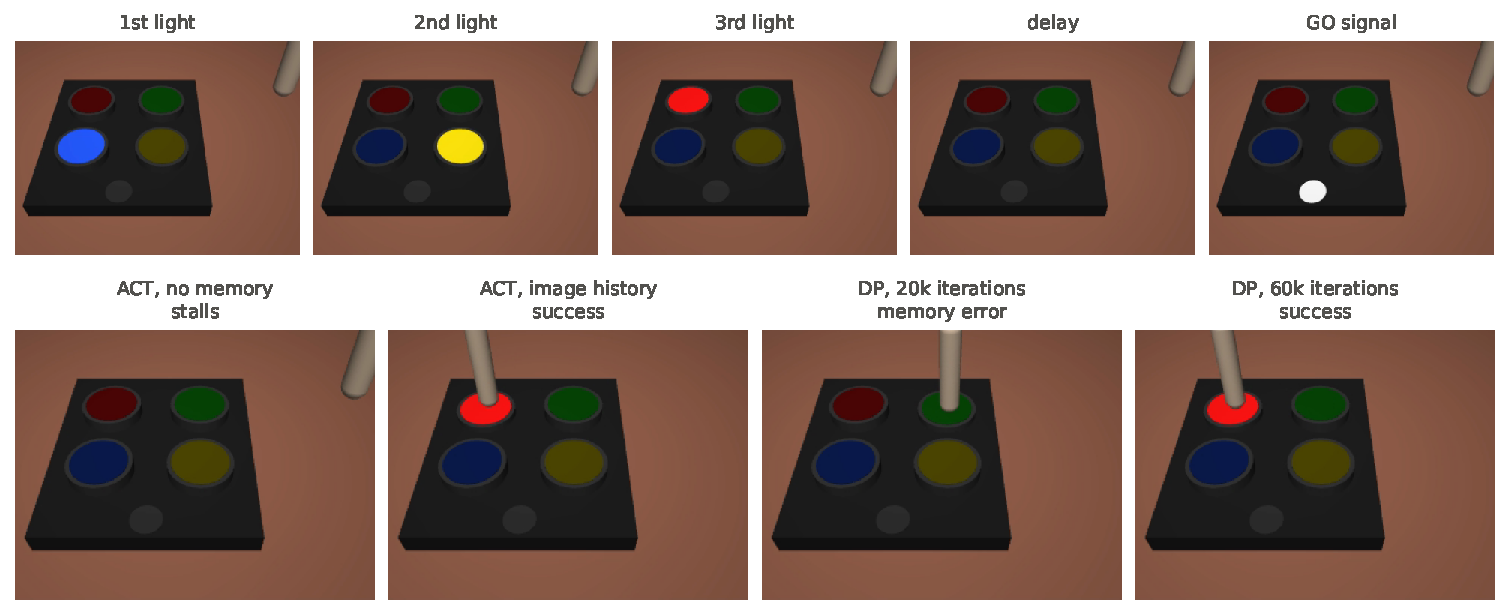
\includegraphics[width=\linewidth]{../figures/teaser.pdf}
  \caption{RoboSimon. Top: presentation of a three-button sequence (blue, yellow, red), delay and GO signal, as seen by the policy. Bottom: last frame of the same test episode for four policies. Without memory, ACT never leaves its rest pose; DP trained for 20k iterations presses blue then green; ACT and DP trained for 60k iterations reproduce the sequence.}
  \label{fig:teaser}
\end{figure}

% =====================================================================
\section{Introduction}

Behaviour cloning policies predict the next actions from the current observation or from a short window of recent ones: ACT~\citep{zhao2023act} uses a single frame per camera and Diffusion Policy~\citep{chi2023diffusion} two. This is enough when everything needed to act is visible, but not when the relevant information has left the field of view, as with an instruction that was shown and then removed. Two identical observations can then call for different actions.

Giving the policy a longer history does not always help. An imitator can exploit spurious correlations in the extra information~\citep{dehaan2019causal}, and when past actions are easy to read from the history it may learn to continue its previous action, failing precisely when the expert changes behaviour; this is the copycat problem of Wen et al.~\citep{wen2020copycat}. Diffusion policies have also been reported to ignore the history they are given~\citep{torne2025ptp}. Existing memory benchmarks~\citep{dai2026robomme} target large vision-language-action models on tasks where manipulation and memory are both difficult, which makes the two sources of failure hard to separate.

We ask whether compact policies trained on a few hundred demonstrations use an image history when the task requires memory, and whether making their past actions easy to read leads to copycat behaviour. To answer this, we introduce RoboSimon, a task in which memory load is controlled and chance level is known exactly; we compare ACT and Diffusion Policy with an identical memory module, so that only the action head differs; and we use behavioural and representational diagnostics under a pre-registered analysis plan. The main finding is that the memory failures and copycat behaviour of Diffusion Policy at the planned budget come from under-training and disappear with three times more iterations.

% =====================================================================
\section{Task, policies and protocol}

\paragraph{RoboSimon.} The scene is simulated in MuJoCo~\citep{todorov2012mujoco}. A board carries four buttons (red, green, blue, yellow) and a white GO light. After 1\,s of rest, a sequence $s\in\{1,\dots,4\}^L$ is presented, each button being lit for 0.6\,s and then off for 0.3\,s. All lights stay off during a 2\,s delay, the GO light then shines for 0.2\,s, and the agent has $3+2.5L$ seconds to press the sequence. The first wrong press, or a press before the end of the GO signal, ends the episode. The agent observes a $240\times320$ image and the position $q_t$ of a finger moved by three position-controlled slide joints, and outputs a target position at 30\,Hz. During execution nothing in the scene indicates the next button, so a policy without access to $s$ succeeds with probability at most $4^{-L}$. A scripted expert, which stays still before the GO signal and then follows minimum-jerk trajectories with random timing and 3\,mm target noise, provides 500 demonstrations per length. The expert solves every episode, and linear probes confirm that neither the scene nor the finger position reveals the sequence after the presentation (Appendix~\ref{app:e0}).

\paragraph{Policies.} All images are encoded by a frozen ResNet-18~\citep{he2016resnet} pre-trained on ImageNet and pooled into a 512-dimensional vector. Freezing the encoder prevents a policy without memory from learning to ignore the lights, which would confound the comparison, and allows the embeddings to be computed once. The memory module receives one frame every 0.2\,s since the start of the episode plus the current frame; each frame is a token made of its projected embedding and a sinusoidal encoding of its age, a two-layer transformer processes the tokens, and four learned queries extract four memory tokens by cross-attention. ACT~\citep{zhao2023act} ($d=512$, CVAE with $\beta=10$) appends the memory tokens to its encoder input; DP~\citep{chi2023diffusion} (1D U-Net with FiLM conditioning~\citep{perez2018film}, DDPM training and 10-step DDIM sampling~\citep{ho2020ddpm,song2021ddim}) concatenates them to its conditioning vector. Both predict 32 actions and execute 16. Full settings are in Appendix~\ref{app:settings}. We compare four variants: B0, without memory; M1, with the image history; M1p, with the image history and the past finger positions, which makes past actions easy to read; and the oracle B1, which receives the sequence together with the image history. The oracle needs the history because the number of buttons already pressed is not visible when a colour repeats, as in $s=(c,c,x)$.

\paragraph{Protocol.} Each condition is trained with three seeds for 20{,}000 iterations, a budget fixed in advance on the loss plateau of B0 and B1. The checkpoint with the best success on 30 validation episodes is evaluated on 100 test episodes, shared by all methods. E1 covers B0, B1 and M1 for both families at $L\in\{2,3,4\}$, and E2 adds M1p at $L=3$. Besides success, we measure an \emph{inertia index}: on the expert's test demonstrations, at each instant where the expert leaves a button for another one, we check whether the predicted chunk is closer to holding the last action than to the expert's chunk. A high index is the signature of copycat behaviour. Confidence intervals at 95\% come from a two-way bootstrap over seeds and episodes~\citep{agarwal2021precipice}. Before E1, we committed three hypotheses with their decision rules: H0, B0 succeeds at chance level; H1, M1 beats B0 by more than 10 points at $L=3$ (C1) and its gap to the oracle grows with $L$ (C2); H2, M1p raises the inertia index and lowers success relative to M1 (C3), more for ACT than for DP (C4).

% =====================================================================
\section{Results}

\subsection{ACT uses the history; DP only partly}

\begin{figure}[t]
  \centering
  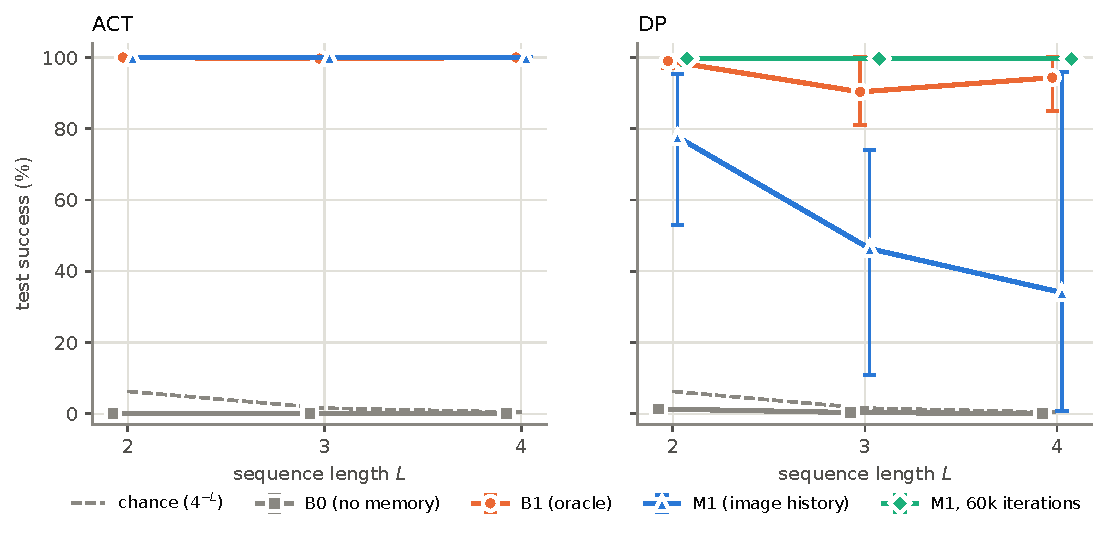
\includegraphics[width=\linewidth]{../figures/success_by_length.pdf}
  \caption{Test success as a function of sequence length (3 seeds, 100 episodes each, 95\% bootstrap intervals). The green curve, DP M1 trained for 60k iterations on new seeds, comes from Section~\ref{sec:budget}.}
  \label{fig:success}
\end{figure}

\begin{table}[t]
  \centering\small
  \caption{Test success in E1 and E2 (\%; 95\% bootstrap intervals below each value).}
  \label{tab:e1}
  \begin{tabular}{lcccccc}
\toprule
Variant & ACT, $L=2$ & ACT, $L=3$ & ACT, $L=4$ & DP, $L=2$ & DP, $L=3$ & DP, $L=4$ \\
\midrule
Chance ($4^{-L}$) & 6.2 & 1.6 & 0.4 & 6.2 & 1.6 & 0.4 \\
B0 & \makecell{0.0\\[-1pt]{\scriptsize [0.0, 0.0]}} & \makecell{0.0\\[-1pt]{\scriptsize [0.0, 0.0]}} & \makecell{0.0\\[-1pt]{\scriptsize [0.0, 0.0]}} & \makecell{1.3\\[-1pt]{\scriptsize [0.0, 3.3]}} & \makecell{0.3\\[-1pt]{\scriptsize [0.0, 2.0]}} & \makecell{0.0\\[-1pt]{\scriptsize [0.0, 0.0]}} \\
B1 & \makecell{100.0\\[-1pt]{\scriptsize [100.0, 100.0]}} & \makecell{99.7\\[-1pt]{\scriptsize [98.0, 100.0]}} & \makecell{100.0\\[-1pt]{\scriptsize [100.0, 100.0]}} & \makecell{99.0\\[-1pt]{\scriptsize [96.7, 100.0]}} & \makecell{90.3\\[-1pt]{\scriptsize [81.0, 100.0]}} & \makecell{94.3\\[-1pt]{\scriptsize [85.0, 100.0]}} \\
M1 & \makecell{100.0\\[-1pt]{\scriptsize [100.0, 100.0]}} & \makecell{100.0\\[-1pt]{\scriptsize [100.0, 100.0]}} & \makecell{100.0\\[-1pt]{\scriptsize [100.0, 100.0]}} & \makecell{77.7\\[-1pt]{\scriptsize [54.0, 95.7]}} & \makecell{46.3\\[-1pt]{\scriptsize [10.0, 75.0]}} & \makecell{34.0\\[-1pt]{\scriptsize [0.7, 96.0]}} \\
M1p & -- & \makecell{99.7\\[-1pt]{\scriptsize [98.0, 100.0]}} & -- & -- & \makecell{29.0\\[-1pt]{\scriptsize [4.0, 59.0]}} & -- \\
\bottomrule
\end{tabular}

\end{table}

Figure~\ref{fig:success} and Table~\ref{tab:e1} summarise E1 and E2. The oracle succeeds in \res{actb1l3} to \res{actb1l2}\% of the episodes with ACT and \res{dpb1l3} to \res{dpb1l2}\% with DP, so the motor part of the task is not a limiting factor. The policy without memory never exceeds chance, although it fails differently in the two families: ACT B0 never presses a button, since without memory it cannot tell the delay from the start of execution and its deterministic output settles between waiting and moving, whereas DP B0 samples one of the two behaviours and often moves during the delay (\res{errdpb0anticipation}\% of early presses at $L=3$).

ACT with an image history succeeds in \res{actm1l2}\% of the episodes at $L=2$, 3 and 4, for every seed. DP with the same history reaches \res{dpm1l2}, \res{dpm1l3} and \res{dpm1l4}\% on average, and its seeds disagree strongly (\res{seedsdpm1l4}\% at $L=4$). Its failures are mostly memory errors (\res{errdpm1memoire}\% of the episodes at $L=3$). The failing seeds are not guessing: their accuracy at each position of a four-button sequence is between 40 and 50\%, above the 25\% chance level but too low to complete the sequence (Appendix, Figure~\ref{fig:serial}).

Under the pre-registered rules, H0 is confirmed. H1 is inconclusive for both families: its first part holds clearly for ACT (C1 = \res{c1act} points) while for DP the lower bound only reaches the threshold (C1 = \res{c1dp}); its second part cannot be observed for ACT, which is at the ceiling for every length, and for DP the gap to the oracle grows with $L$ without the interval excluding zero (C2 = \res{c2dp}).

\subsection{Copycat behaviour appears only in under-trained DP}

\begin{figure}[t]
  \centering
  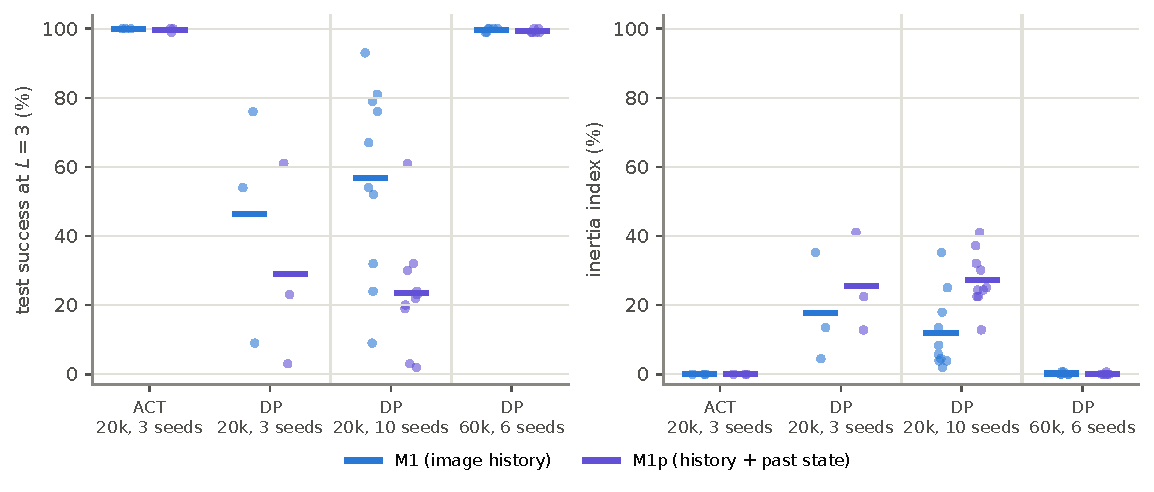
\includegraphics[width=\linewidth]{../figures/copycat.pdf}
  \caption{Test success and inertia index at $L=3$ with the image history (M1) and with the image history and past positions (M1p). Each dot is a seed and each bar a mean. From left to right: protocol (3 seeds), DP with the exploratory extension to 10 seeds, and DP trained for 60k iterations.}
  \label{fig:copycat}
\end{figure}

The past finger positions have no effect on ACT (Figure~\ref{fig:copycat}): M1p succeeds in \res{actm1pl3}\% of the episodes and its inertia index is zero, as for M1. A likely reason is that a chunk of 32 actions has to cover the whole movement to the next button, so continuing the current motion is costly in the loss, and that the next button can be read without ambiguity from the image history. For DP, the three seeds of the protocol point towards copycat behaviour without being conclusive (success \res{c3sdp} points, inertia \res{c3idp} points). H2 is therefore refuted for ACT and inconclusive for DP, and the prediction that ACT would be more affected is contradicted.

Since three seeds were too few, we trained seven more seeds of DP M1 and M1p after E1 and E2; this exploratory extension was not pre-registered and does not change the verdicts. With ten seeds the effect becomes clear: the past positions change success by \res{xsuccessdiff} points and the inertia index by \res{xinertiadiff} points, and across the twenty seeds the inertia index is strongly correlated with failure ($r=\res{corrinertia}$). A counterfactual test, in which the presented sequence is replaced by another one, and linear probes on the memory tokens give a consistent picture (Appendix~\ref{app:diag}): ACT stores the sequence and follows it in every episode, while under-trained DP seeds store it less well and follow it less often, all the more when they see their past positions.

\subsection{Diffusion Policy was under-trained}
\label{sec:budget}

\begin{figure}[t]
  \centering
  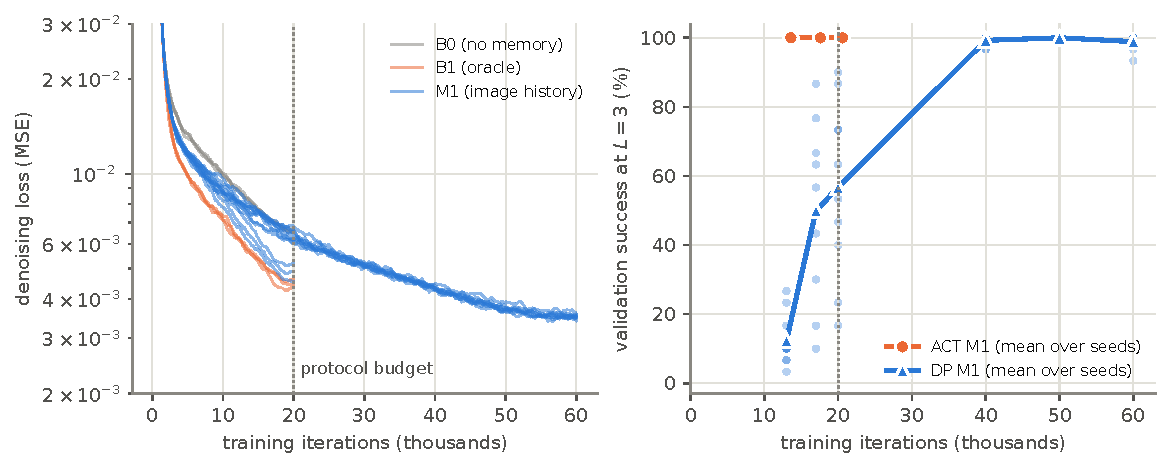
\includegraphics[width=\linewidth]{../figures/learning_curves.pdf}
  \caption{DP at $L=3$. Left: training loss of B0, B1 and M1, one line per run; the M1 runs that continue beyond 20k iterations are those of the follow-up study. Right: validation success of M1 at each evaluated checkpoint (dots: seeds; line: mean), with ACT M1 for comparison.}
  \label{fig:learning}
\end{figure}

To find why DP fails where ACT does not, we ran a follow-up study outside the pre-registered protocol, with its selection rule and confirmation contrast committed before the confirmation runs. A pilot on three seeds at $L=3$ compared four candidates on validation episodes only: a single observation frame, so that DP cannot infer its destination from the finger's velocity; past-token prediction~\citep{torne2025ptp}, which makes the policy also denoise its 16 previous actions; 60k training iterations instead of 20k; and the combination of the last two. The selected method was then trained on six new seeds.

\begin{table}[t]
  \centering\small
  \caption{Follow-up study. Top: pilot (DP M1, $L=3$, seeds 0 to 2), selection on validation, ties within 5 points broken in favour of the simplest method. Bottom: confirmation of the selected method on new seeds (\%).}
  \label{tab:budget}
  \begin{tabular}{lccc}
\toprule
Candidate & Validation per seed (\%) & Validation mean & Test (\%) \\
\midrule
DP, 20k iterations (E1) & 17, 47, 63 & 42 & 46.3 [11.0, 74.0] \\
DP, single observation frame & 13, 23, 80 & 39 & 36.3 [11.7, 75.0] \\
DP + PTP & 3, 63, 47 & 38 & 30.3 [1.0, 58.0] \\
DP, 60k iterations & 100, 100, 100 & 100 & 98.3 [95.0, 100.0] \\
DP + PTP, 60k iterations & 100, 100, 100 & 100 & 98.0 [94.7, 100.0] \\
\bottomrule
\end{tabular}

  \vspace{6pt}

  \begin{tabular}{lrrcr}
\toprule
Variant & $L$ & Seeds & Test success (\%) & Inertia (\%) \\
\midrule
M1 & 2 & 3 & 99.7 [98.0, 100.0] & -- \\
M1 & 3 & 6 & 99.7 [98.7, 100.0] & 0.2 \\
M1 & 4 & 3 & 99.7 [98.7, 100.0] & -- \\
M1p & 3 & 6 & 99.3 [98.0, 100.0] & 0.1 \\
\bottomrule
\end{tabular}

\end{table}

Only the longer training mattered (Table~\ref{tab:budget}). With 60k iterations, DP reached \res{pilotvaldp60k}\% on validation for all three seeds, against \res{pilotvaldp20k}\% at 20k; past-token prediction added nothing, and a single frame did not help (\res{pilotvaldpo120k}\%). Following the rule, we kept plain DP with 60k iterations. On the new seeds it succeeds in \res{confm1l2}, \res{confm1l3} and \res{confm1l4}\% of the episodes at $L=2,3,4$, and M1p in \res{confm1pl3}\%. The pre-registered contrast with E1 is \res{aone} points, above the predicted 10 points, and the past positions no longer have any effect (\res{atwos} points in success, \res{atwoi} in inertia; inertia index \res{confinertiam1}\%).

Figure~\ref{fig:learning} shows why 20k iterations looked sufficient. The training loss of B0, B1 and M1 has flattened by then, but the validation success of M1 is only \res{lcdptwenty}\% on average at 20k iterations and reaches \res{lcdpforty}\% at 40k. Most of the denoising loss is spent on the shape of the movements, which all variants learn at the same pace; choosing the right button is a small part of the loss and is learned later. ACT M1 is already at 100\% at its first checkpoint. The copycat behaviour of DP was therefore a stage of learning, not a property of the diffusion head.

% =====================================================================
\section{Discussion}

Both policy families can solve RoboSimon with an image history; they differ in how fast they learn to do so. In the range of lengths studied, the gap to the oracle measured in E1 reflects this speed rather than a capacity limit. Wen et al.~\citep{wen2020copycat} studied single-step policies; with 32-action chunks, repeating the last action is penalised over the whole chunk, which may explain why ACT never shows copycat behaviour, in line with the argument of Zhao et al.~\citep{zhao2023act} that chunking shortens the effective horizon. For DP, copycat behaviour is what remains before the policy has learned to read its memory, and the inertia index measures how far a seed is from that point. Past-token prediction, which Torne et al.~\citep{torne2025ptp} found useful for long contexts, brought nothing here, where episodes last 10 to 20\,s and the history is sub-sampled. Coverage of the sequence space~\citep{sobolmark2026bpp} was not limiting either: 229 of the 256 sequences of length 4 appear in the training data, and ACT also solves the 11 test sequences that do not.

The study has clear limits. The effector is a Cartesian finger, so motor difficulty, which could interact with memory on a real arm, is absent; we used a single frozen encoder and a single memory architecture; the ten-seed extension was decided after seeing the first results; and the protocol budget, set on the loss of policies without memory, was too short for DP, so the E1 and E2 results for DP describe the method at that budget rather than its limit.

% =====================================================================
\section{Conclusion}

On RoboSimon, a compact ACT policy reading a sub-sampled image history with attention reproduces sequences of two to four buttons without error, from 500 demonstrations and a frozen encoder. Diffusion Policy with the same memory module reaches the same level after three times as many training iterations; before that, it fails often, varies between seeds and tends to repeat its previous motion. Because its training loss flattens long before it uses its memory, a budget chosen on the loss of policies without memory can make a working architecture look as if it lacked memory. Comparisons of memory mechanisms should therefore fix the budget on a memory variant or report success along training. Natural next steps are learning curves for every length, a recurrent memory module, varying the delay, end-to-end encoder training, and an articulated arm in simulation and then on a real robot.

\bibliographystyle{unsrtnat}
\bibliography{references}

% =====================================================================
\appendix
\section{Validation of the testbed}
\label{app:e0}

\begin{figure}[h]
  \centering
  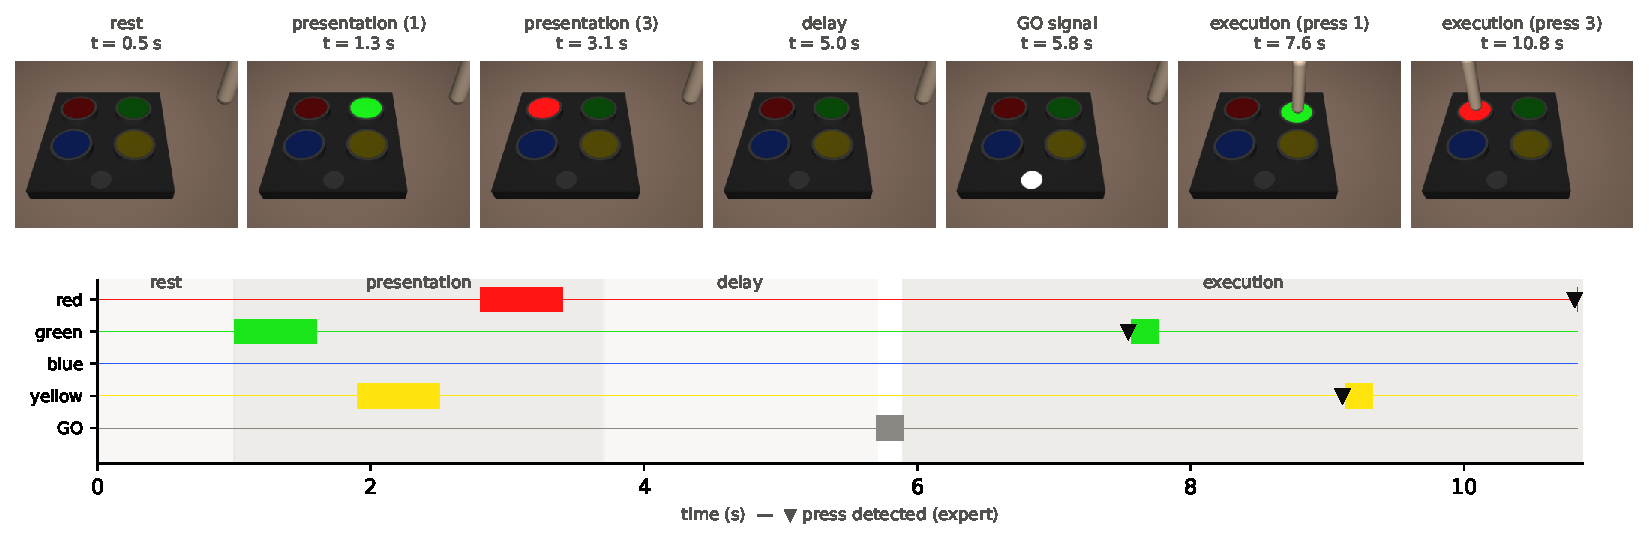
\includegraphics[width=\linewidth]{../figures/scene_timeline.pdf}
  \caption{An episode with $L=3$: camera frames at the main phases, and state of the lights over time; triangles mark the presses of the scripted expert.}
  \label{fig:scene}
\end{figure}

\begin{table}[h]
  \centering\small
  \caption{Validation of the testbed. For B0 and B1, 95\% bootstrap intervals over 3 seeds and 100 test episodes. $^\dagger$A probe on a random execution frame reads the expert's finger, which is often on or moving towards $s_1$; on the first execution frame, before the finger moves, it is at chance.}
  \label{tab:e0}
  \begin{tabular}{llll}
\toprule
Check & Result & Criterion & Verdict \\
\midrule
Scripted expert (500 episodes per $L$) & 100.0, 100.0, 100.0 \% & $\geq 99$\% & pass \\
Determinism (same seed and actions) & bit-identical & identical & pass \\
LED state decoding from $E_h$ (6 classes) & 100.0 \% ($g=1$) & $\geq 99$\% & pass, $g=1$ \\
Leak, random execution frame$^\dagger$ & 39.0 \% ($p=4.9\times10^{-10}$) & not $>25$\% & see text \\
Leak, first execution frame (finger at rest) & 22.5 \% ($p=0.89$) & not $>25$\% & pass \\
Leak, finger state at GO & 24.8 \% ($p=0.57$) & not $>25$\% & pass \\
Positive control, first presentation frame & 100.0 \% ($p=1.5\times10^{-241}$) & $>25$\% expected & pass \\
ACT B0, $L=2$ & 0.0 [0.0, 0.0] \% & not above 6.2\% & pass \\
ACT B0, $L=3$ & 0.0 [0.0, 0.0] \% & not above 1.6\% & pass \\
ACT B1, $L=3$ & 99.7 [98.0, 100.0] \% & $\geq 90$\% & pass \\
DP B0, $L=2$ & 1.3 [0.0, 3.3] \% & not above 6.2\% & pass \\
DP B0, $L=3$ & 0.3 [0.0, 2.0] \% & not above 1.6\% & pass \\
DP B1, $L=3$ & 90.3 [81.0, 100.0] \% & $\geq 90$\% & pass \\
\bottomrule
\end{tabular}

\end{table}

\begin{table}[h]
  \centering\small
  \caption{Sanity checks on 10 training episodes at $L=2$ (3{,}000 iterations). The last column is the largest change in the predicted actions when the presentation frames are replaced; it must be zero for B0 and positive for the other variants.}
  \label{tab:unit}
  \begin{tabular}{lrrr}
\toprule
Policy & Final loss & Success (\%) & $\max|\Delta a|$ \\
\midrule
ACT B0 & 0.0863 & 0 & 0.000 \\
ACT B1 & 0.0651 & 100 & 0.294 \\
ACT M1 & 0.0576 & 100 & 0.325 \\
ACT M1p & 0.0566 & 100 & 0.190 \\
DP B0 & 0.0031 & 0 & 0.000 \\
DP B1 & 0.0029 & 100 & 0.128 \\
DP M1 & 0.0033 & 100 & 0.122 \\
DP M1p & 0.0028 & 100 & 0.082 \\
\bottomrule
\end{tabular}

\end{table}

\section{Settings}
\label{app:settings}

\begin{table}[h]
  \centering\small
  \caption{Action heads. Both use dropout 0.1, batches of 64 and gradient clipping at 10. For ACT, the learning rate of $10^{-5}$ used in LeRobot~\citep{cadene2024lerobot} did not reach a plateau within the budget and was raised to $10^{-4}$, as the protocol prescribed.}
  \label{tab:heads}
  \begin{tabular}{p{2.3cm}p{6.5cm}p{6.5cm}}
    \toprule
    & ACT & Diffusion Policy \\
    \midrule
    Backbone & transformer, $d=512$, 8 heads, 4 encoder and 1 decoder layers & 1D U-Net with channels (256, 512, 1024), kernel 5, FiLM \\
    Generative model & CVAE~\citep{sohn2015cvae}, latent dimension 32, $\beta=10$, $z=0$ at test time & DDPM, 100 steps, cosine schedule~\citep{nichol2021improved}; DDIM, 10 steps \\
    Observation & 1 frame and $q_t$ & 2 frames, $q_{t-1}$ and $q_t$ \\
    Optimiser & AdamW, learning rate $10^{-4}$ & Adam, learning rate $10^{-4}$, cosine decay \\
    Horizon & 32 predicted, 16 executed & 32 predicted, 16 executed \\
    \bottomrule
  \end{tabular}
\end{table}

Three checkpoints in the second half of training are evaluated on validation episodes~\citep{mandlekar2021matters}; at test time the policy runs from the first frame and is queried every 16 steps. The inertia index uses the 156 instants at $L=3$ where the expert leaves a button for a different one. Contrasts are differences in percentage points with two-way bootstrap intervals (10{,}000 resamples), episodes being resampled jointly for the compared methods; no correction for multiple comparisons is applied.

\begin{table}[h]
  \centering\small
  \caption{Contrasts declared before E1 (percentage points, 95\% bootstrap intervals).}
  \label{tab:contrasts}
  \begin{tabular}{llcc}
\toprule
 & Contrast & ACT & DP \\
\midrule
C1 & M1 $-$ B0 at $L=3$ & +100.0 [100.0, 100.0] & +46.0 [10.0, 75.0] \\
C2 & $(\text{B1}-\text{M1})_{L=4} - (\text{B1}-\text{M1})_{L=2}$ & +0.0 [0.0, 0.0] & +39.0 [$-$20.7, 87.0] \\
C3 & M1p $-$ M1 at $L=3$, success & $-$0.3 [$-$2.0, 0.0] & $-$17.3 [$-$57.0, 26.3] \\
C3 & M1p $-$ M1 at $L=3$, inertia & +0.0 [0.0, 0.0] & +7.7 [$-$12.8, 28.2] \\
C4 & $(\text{M1p}-\text{M1})_{\text{ACT}} - (\text{M1p}-\text{M1})_{\text{DP}}$ & success +17.0 [$-$26.3, 57.3] & inertia $-$7.7 [$-$27.6, 13.0] \\
\bottomrule
\end{tabular}

\end{table}

\section{Diagnostics}
\label{app:diag}

The \emph{counterfactual following rate} replaces the presentation frames by those of a sequence $s'$ with $s'_1\neq s_1$ and measures how often the first press is $s'_1$. \emph{Linear probes}~\citep{alain2016probes} predict each element of the sequence from the memory tokens at the GO signal (five-fold cross-validation over episodes). With 100 episodes for 1{,}024 features, the probes underestimate the information present: one DP seed follows the substituted sequence in 98\% of the episodes while the probe decodes its first element in only 56\%.

\begin{figure}[h]
  \centering
  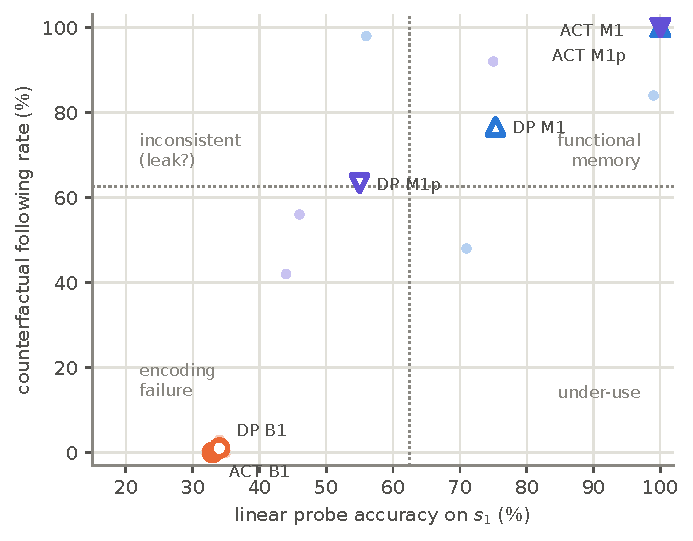
\includegraphics[width=0.48\linewidth]{../figures/probes_vs_following.pdf}\hfill
  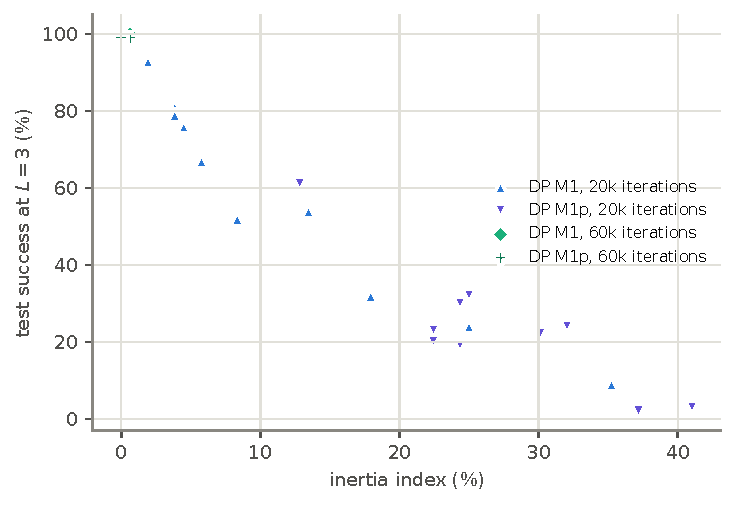
\includegraphics[width=0.5\linewidth]{../figures/inertia_by_seed.pdf}
  \caption{Left: probe accuracy on $s_1$ against the counterfactual following rate at $L=3$ (large markers: means, filled for ACT and open for DP; small dots: seeds). Right: DP, one point per seed, inertia index against test success after 20k and 60k iterations.}
  \label{fig:diag}
\end{figure}

\begin{figure}[h]
  \centering
  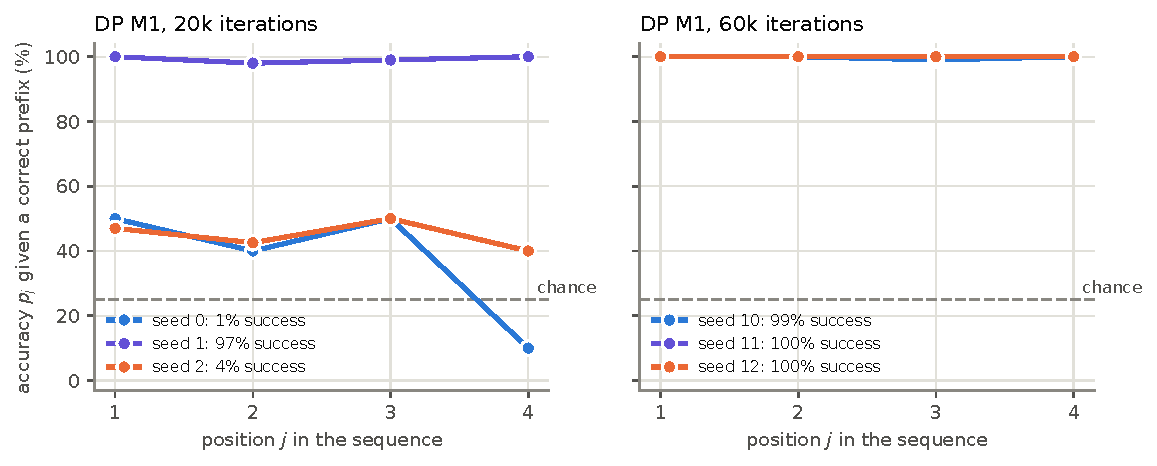
\includegraphics[width=\linewidth]{../figures/serial_position.pdf}
  \caption{Accuracy at each position of a four-button sequence, given a correct prefix, for each seed of DP M1, after 20k iterations (left) and 60k iterations (right).}
  \label{fig:serial}
\end{figure}

\begin{table}[h]
  \centering\small
  \caption{Diagnostics at $L=3$, averaged over seeds (\%).}
  \label{tab:diag}
  \begin{tabular}{llrcrr}
\toprule
Family & Variant & Inertia & Probe $s_1/s_2/s_3$ & Following & $P(\text{1st}=s_1)$ \\
\midrule
ACT & B0 & 100.0 & -- & -- & -- \\
ACT & B1 & 0.4 & 33 / 22 / 25 & 0.0 & 99.7 \\
ACT & M1 & 0.0 & 100 / 74 / 68 & 100.0 & 0.0 \\
ACT & M1p & 0.0 & 100 / 78 / 74 & 100.0 & 0.0 \\
DP & B0 & 73.7 & -- & -- & -- \\
DP & B1 & 0.9 & 34 / 29 / 31 & 1.0 & 96.7 \\
DP & M1 & 17.7 & 75 / 38 / 37 & 76.7 & 6.3 \\
DP & M1p & 25.4 & 55 / 38 / 32 & 63.3 & 8.3 \\
\bottomrule
\end{tabular}

\end{table}

\begin{table}[h]
  \centering\small
  \caption{Exploratory extension: DP at $L=3$ with 10 seeds (\%, 95\% bootstrap intervals; not pre-registered).}
  \label{tab:exploratory}
  \begin{tabular}{lccc}
\toprule
 & M1 (10 seeds) & M1p (10 seeds) & M1p $-$ M1 \\
\midrule
Success (\%) & 56.7 [39.1, 72.4] & 23.6 [14.0, 34.3] & $-$33.1 [$-$51.9, $-$13.6] \\
Inertia index (\%) & 12.0 [5.8, 19.7] & 27.2 [21.3, 33.3] & +15.2 [6.4, 23.8] \\
Probe $s_1$ / following (\%) & 89 / 84 & 54 / 67 &  \\
\bottomrule
\end{tabular}

\end{table}

\section{Per-seed results and compute}

\begin{table}[h]
  \centering\small
  \caption{Outcome of the test episodes at $L=3$ (\% of 300 episodes).}
  \label{tab:outcomes}
  \begin{tabular}{llrrrrrr}
\toprule
Family & Variant & Success & Memory & Repetition & Motor & Stall & Early press \\
\midrule
ACT & B0 & 0.0 & 0.0 & 0.0 & 0.0 & 100.0 & 0.0 \\
ACT & B1 & 99.7 & 0.3 & 0.0 & 0.0 & 0.0 & 0.0 \\
ACT & M1 & 100.0 & 0.0 & 0.0 & 0.0 & 0.0 & 0.0 \\
ACT & M1p & 99.7 & 0.0 & 0.3 & 0.0 & 0.0 & 0.0 \\
DP & B0 & 0.3 & 28.3 & 4.7 & 0.0 & 0.7 & 66.0 \\
DP & B1 & 90.3 & 5.0 & 4.0 & 0.3 & 0.3 & 0.0 \\
DP & M1 & 46.3 & 46.0 & 6.7 & 0.7 & 0.3 & 0.0 \\
DP & M1p & 29.0 & 63.3 & 7.7 & 0.0 & 0.0 & 0.0 \\
\bottomrule
\end{tabular}

\end{table}

\begin{table}[h]
  \centering\small
  \caption{Test success per seed (\%) and selected checkpoint.}
  \label{tab:seeds}
  \begin{tabular}{llrrrrl}
\toprule
Family & Variant & $L$ & Seed 0 & Seed 1 & Seed 2 & Selected checkpoint \\
\midrule
ACT & B0 & 2 & 0 & 0 & 0 & 20k, 20k, 20k \\
ACT & B0 & 3 & 0 & 0 & 0 & 20k, 20k, 20k \\
ACT & B0 & 4 & 0 & 0 & 0 & 20k, 20k, 20k \\
ACT & B1 & 2 & 100 & 100 & 100 & 20k, 20k, 20k \\
ACT & B1 & 3 & 100 & 100 & 99 & 20k, 20k, 20k \\
ACT & B1 & 4 & 100 & 100 & 100 & 20k, 20k, 20k \\
ACT & M1 & 2 & 100 & 100 & 100 & 20k, 20k, 20k \\
ACT & M1 & 3 & 100 & 100 & 100 & 20k, 20k, 20k \\
ACT & M1 & 4 & 100 & 100 & 100 & 20k, 20k, 20k \\
ACT & M1p & 3 & 99 & 100 & 100 & 16k, 20k, 20k \\
DP & B0 & 2 & 1 & 1 & 2 & 20k, 13k, 20k \\
DP & B0 & 3 & 1 & 0 & 0 & 20k, 20k, 16k \\
DP & B0 & 4 & 0 & 0 & 0 & 20k, 13k, 13k \\
DP & B1 & 2 & 100 & 99 & 98 & 20k, 20k, 20k \\
DP & B1 & 3 & 100 & 82 & 89 & 20k, 20k, 16k \\
DP & B1 & 4 & 85 & 100 & 98 & 20k, 20k, 16k \\
DP & M1 & 2 & 96 & 52 & 85 & 20k, 20k, 20k \\
DP & M1 & 3 & 9 & 54 & 76 & 20k, 20k, 20k \\
DP & M1 & 4 & 1 & 97 & 4 & 16k, 20k, 16k \\
DP & M1p & 3 & 3 & 23 & 61 & 16k, 20k, 16k \\
\bottomrule
\end{tabular}

\end{table}

\begin{table}[h]
  \centering\small
  \caption{Diagnostics per seed at $L=3$ (protocol, 20k iterations; \%).}
  \label{tab:diagseeds}
  \begin{tabular}{llrrrrr}
\toprule
Family & Variant & Seed & Probe $s_1$ & Following & Inertia & Success \\
\midrule
ACT & M1 & 0 & 100 & 100 & 0 & 100 \\
ACT & M1 & 1 & 100 & 100 & 0 & 100 \\
ACT & M1 & 2 & 100 & 100 & 0 & 100 \\
ACT & M1p & 0 & 100 & 100 & 0 & 99 \\
ACT & M1p & 1 & 100 & 100 & 0 & 100 \\
ACT & M1p & 2 & 100 & 100 & 0 & 100 \\
DP & M1 & 0 & 71 & 48 & 35 & 9 \\
DP & M1 & 1 & 99 & 84 & 13 & 54 \\
DP & M1 & 2 & 56 & 98 & 4 & 76 \\
DP & M1p & 0 & 44 & 42 & 41 & 3 \\
DP & M1p & 1 & 46 & 56 & 22 & 23 \\
DP & M1p & 2 & 75 & 92 & 13 & 61 \\
\bottomrule
\end{tabular}

\end{table}

\begin{table}[h]
  \centering\small
  \caption{Compute on RTX 5070 GPUs, measured per process; two or three conditions shared each GPU, so these figures overestimate GPU time.}
  \label{tab:compute}
  \begin{tabular}{lrrr}
\toprule
Set & Conditions & Training (h) & Total (h) \\
\midrule
Protocol (E1, E2) & 60 & 20.7 & 22.4 \\
Exploratory extension & 14 & 7.5 & 8.1 \\
DP improvement, pilot & 12 & 8.3 & 8.7 \\
DP improvement, confirmation & 18 & 19.9 & 20.5 \\
\bottomrule
\end{tabular}

\end{table}

\begin{sloppypar}
\noindent The repository contains the code, the episode lists and the result of every evaluated episode; \texttt{analyse.py} produces every figure, table and number of this report from these results. The hypotheses and the rules of the follow-up study were committed before the corresponding experiments (\texttt{preenregistrement.md}, \texttt{preenregistrement\_amelioration.md}).
\end{sloppypar}

\end{document}
